%%%%%%%%%%%%%%%%%%%%%%%%%%%%%%%%%%%%%%%%%
% FRI Data Science_report LaTeX Template
% Version 1.0 (28/1/2020)
% 
% Jure Demšar (jure.demsar@fri.uni-lj.si)
%
% Based on MicromouseSymp article template by:
% Mathias Legrand (legrand.mathias@gmail.com) 
% With extensive modifications by:
% Antonio Valente (antonio.luis.valente@gmail.com)
%
% License:
% CC BY-NC-SA 3.0 (http://creativecommons.org/licenses/by-nc-sa/3.0/)
%
%%%%%%%%%%%%%%%%%%%%%%%%%%%%%%%%%%%%%%%%%


%----------------------------------------------------------------------------------------
%	PACKAGES AND OTHER DOCUMENT CONFIGURATIONS
%----------------------------------------------------------------------------------------
\documentclass[fleqn,moreauthors,10pt]{ds_report}
\usepackage[english]{babel}
\usepackage{comment}

\graphicspath{{fig/}}



%----------------------------------------------------------------------------------------
%	ARTICLE INFORMATION
%----------------------------------------------------------------------------------------

% Header
\JournalInfo{FRI Natural language processing course 2023}

% Interim or final report
\Archive{Project report} 
%\Archive{Final report} 

% Article title
\PaperTitle{Project 3: Paraphrasing sentences} 

% Authors (student competitors) and their info
\Authors{Matjaž Zupančič Muc, Marko Novak, and Klemen Laznik}

% Advisors
\affiliation{\textit{Advisers: Slavko Žitnik}}

% Keywords
\Keywords{Sentence paraphrasing, }
\newcommand{\keywordname}{Keywords}


%----------------------------------------------------------------------------------------
%	ABSTRACT
%----------------------------------------------------------------------------------------


\Abstract{
The abstract goes here. The abstract goes here. The abstract goes here. The abstract goes here. The abstract goes here. The abstract goes here. The abstract goes here. The abstract goes here. The abstract goes here. The abstract goes here. The abstract goes here. The abstract goes here. The abstract goes here. The abstract goes here. The abstract goes here. The abstract goes here. The abstract goes here. The abstract goes here. The abstract goes here. The abstract goes here. The abstract goes here. The abstract goes here. The abstract goes here. The abstract goes here. The abstract goes here. The abstract goes here.
}

%----------------------------------------------------------------------------------------

\begin{document}

% Makes all text pages the same height
\flushbottom

% Print the title and abstract box
\maketitle

% Removes page numbering from the first page
\thispagestyle{empty}

%----------------------------------------------------------------------------------------
%	ARTICLE CONTENTS
%----------------------------------------------------------------------------------------

\section*{Introduction}

\begin{comment}
These latex files are intended to serve as a the template for the NLP course at FRI.  The template is adapted from the FRI Data Science Project Competition. template  If you find mistakes in the template or have problems using it, please consult Jure Demšar (\href{mailto:jure.demsar@fri.uni-lj.si}{jure.demsar@fri.uni-lj.si}). In the Introduction section you should write about the relevance of your work (what is the purpose of the project, what will we solve) and about related work (what solutions for the problem already exist). Where appropriate, reference scientific work conducted by other researchers. For example, the work done by Demšar et al. \cite{Demsar2016BalancedMixture} is very important for our project. The abbreviation et al. is for et alia, which in latin means and others, we use this abbreviation when there are more than two authors of the work we are citing. If there are two authors (or if there is a single author) we just write down their surnames. For example, the work done by Demšar and Lebar Bajec \cite{Demsar2017LinguisticEvolution} is also important for successful completion of our project.
\end{comment}

Paraphrasing plays an important role in language understanding tasks, such as question answering, machine translation and semantic parsing. Additionally, it serves as a useful method for data augmentation. The goal of paraphrase generation is to produce alternative versions of a given sentence that may feature different phrasing or structure, yet still accurately convey the original meaning. Creating high-quality paraphrases is a challenging problem in natural language processing (NLP), as it requires a deep understanding of the underlying semantics and syntax of the input sentence. In recent years, there has been a growing interest in using machine learning techniques, particularly transformer models, to automatically generate paraphrases.

Authors of \cite{federmann-etal-2019-multilingual} compare translation based paraphrase gathering using human (experts and non-experts), automatic and hybrid techniques. The automatic technique is based on back translation using a neural machine translation (NMT) model. They first translate a source sentence from one language to multiple target languages (i.e pivot languages) and than back to the original language. They found that NMT based paraphrases have a higher diversity compared to
paraphrases written by human non experts, but NMT based paraphrases don't reach the adequacy or fluency level provided by expert paraphrases. They found that NMTs corrupt inputs such as slang and typing errors leading to bad paraphrases. They also found that NMTs struggle with negation, i.e NMTs tend to loose or add negation to a sentence. Finally they found that paraphrases generated by pivot languages which are closely related have a higher adequacy and fluency level, while paraphrases generated by pivot languages that are not closely related have higher diversity. They conclude that NMT based paraphrase generation is cheap and diverse, although NMTs produce less fluent outputs post editing could be used to improve the quality with little additional expenditure.

Existing paraphrase generating language models build on large sequence-to-sequence / encoder-decoder language models. The general principle of those models is similar to models used in machine translations where the first part of the model creates an encoded representation of the input, and the decoder part generates a new sequence from the encoding. However, while machine translation models are trained to generate an output which closely represents the input sentence, for paraphrasing the output needs to differ from the input while maintaining information. In {Paraphrase Generation: A Survey of the State of the Art}~\cite{zhou-bhat-2021-paraphrase}, the authors present several improvements on top of the encoder-decoder models, which are used by the current state-of-the-art models to achieve better results. 

\textbf{Attention} mechanism helps models emphasise the important information within the input. This information is passed to the decoder part of the model as an extra input vector. On the other hand, the \textbf{copy} mechanism helps determine whether to generate a new token or copy an input token at each step of decoding. This helps to improve the form of generated paraphrases, but limits the diversity of generated text. The two common approaches to improve the diversity of generated paraphrases are \textbf{variational autoencoders} (VAE) and \textbf{reinforcement learning} (RL); the benefit of using RL with a pretrained language model is that it doesn't require a large labelled dataset and can perform paraphrasing in unsupervised setting. The models trainde this way have also demonstrated the ability to perform cross-lingual transfer without additional finetuning~\cite{DBLP:journals/corr/abs-2010-12885}.

\textbf{Paraphrase evaluation} is a challenging problem, and existing metrics have limitations. In this paper~\cite{evaluation-metrics-in-paraphrase-generation}, the authors propose a new metric named ParaScore, which takes into account both semantic similarity and lexical divergence between the input sentence and candidate paraphrases. ParaScore is a reference-based metric and is defined as the maximum value between the semantic similarity of the candidate paraphrase to the reference paraphrase and the input sentence to the reference paraphrase, plus a weighted measure of lexical divergence. The authors also propose a reference-free version of ParaScore by removing the reference paraphrase from the metric.

The authors conducted experiments on four datasets and compared ParaScore to several baselines, including BLEU, Rouge, METEOR, BERT-iBLEU, and iBLEU. The results show that ParaScore performs significantly better than all the other metrics on all the datasets and is more robust than other metrics.

The proposed metric addresses some of the limitations of existing metrics, such as BLEU, which is a widely used metric but does not consider lexical divergence, and iBLEU, which considers lexical divergence but is sub-optimal. ParaScore provides a better evaluation of paraphrasing and has the potential to be used in applications such as text simplification and data augmentation.



%% 

%------------------------------------------------

\section*{Methods}

Given instructions, the proposed pipeline is as follows: Get/use an existing dataset (ccGigafida, ccKres, …). We might be able to use {Slovenian datasets for contextual synonym and antonym detection}~\cite{11356/1694} to obtain synonyms which could be used to generate paraphrased sentences from other corpora. Use Slovene NMTs to generate the dataset of paraphrases with first reference in mind.

 We could evaluate the quality of the dataset generated by NMTs using contextual similarity between original sentence and the paraphrased sentence. To do this we would embed the sentences using BERT and than compute the cosine similarity between the embeddings. We can use a readability score such as the Flesch Reading Ease score or the Gunning Fog Index to evaluate the clarity of the paraphrased sentences. To estimate the fluency we could use large language models such as BERT and GPT. BERT and GPT can be used to generate fluency scores based on the model's prediction of the likelihood of the sentence being a natural language sentence. Because fluency is closely related to grammatical correctness and syntax we check for grammar and syntax errors. [This point is yet to be decided, we proposed a similar approach to ParaScore (\textbf{caution:} this would require tuning to make useful, which is not suitable for this stage of the pipeline), we can calculate similarity using many different calculations, like Pearson, Spearman, Cosine etc. We can use a readability score such as the Flesch Reading Ease score or the Gunning Fog Index to evaluate the clarity of the paraphrased sentences. For fluency I have 0 idea, sounds way too complex to calculate for being suggested as a manual method. Of course we can always use a small subgroup and evaluate by hand e.g. human evaluation.]

 We'll train a baseline sequence to sequence T5 model on top of the generated dataset. We could use random pattern embeddings or add a diversity term to the loss function to increase the diversity of generated paraphrases. We also consider using a multilingual base model, as it would allow us to also use existing datasets from other languages and transfer that knowledge to Slovenian language.

\textbf{Regarding the use of ParaScore:} Given the width of the study~\cite{evaluation-metrics-in-paraphrase-generation}, we are lead to believe that for the task at hand - paraphrasing sentences, the existing metrics are insufficient in handling neither lexical diverging, nor semantic similarity simultaneously, which are both present. We should also be aware of potential drawback since we introduce a hyper-parameter in need of tuning. The idea behind using ParaScore is mainly to evaluate the quality of our paraphrasing model but are keen to use a similar approach to evaluate the NMTs output, which is the input - data for model training.

 

\begin{comment}
Use the Methods section to describe what you did an how you did it -- in what way did you prepare the data, what algorithms did you use, how did you test various solutions ... Provide all the required details for a reproduction of your work.Below are \LaTeX examples of some common elements that you will probably need when writing your report (e.g. figures, equations, lists, code examples ...).


\subsection*{Equations}

You can write equations inline, e.g. $\cos\pi=-1$, $E = m \cdot c^2$ and $\alpha$, or you can include them as separate objects. The Bayes’s rule is stated mathematically as:

\begin{equation}
	P(A|B) = \frac{P(B|A)P(A)}{P(B)},
	\label{eq:bayes}
\end{equation}

where $A$ and $B$ are some events. You can also reference it -- the equation \ref{eq:bayes} describes the Bayes's rule.

\subsection*{Lists}

We can insert numbered and bullet lists:

% the [noitemsep] option makes the list more compact
\begin{enumerate}[noitemsep]
	\item First item in the list.
	\item Second item in the list.
	\item Third item in the list.
\end{enumerate}

\begin{itemize}[noitemsep]
	\item First item in the list.
	\item Second item in the list.
	\item Third item in the list.
\end{itemize}

We can use the description environment to define or describe key terms and phrases.

\begin{description}
	\item[Word] What is a word?.
	\item[Concept] What is a concept?
	\item[Idea] What is an idea?
\end{description}


\subsection*{Random text}

This text is inserted only to make this template look more like a proper report. Lorem ipsum dolor sit amet, consectetur adipiscing elit. Etiam blandit dictum facilisis. Lorem ipsum dolor sit amet, consectetur adipiscing elit. Interdum et malesuada fames ac ante ipsum primis in faucibus. Etiam convallis tellus velit, quis ornare ipsum aliquam id. Maecenas tempus mauris sit amet libero elementum eleifend. Nulla nunc orci, consectetur non consequat ac, consequat non nisl. Aenean vitae dui nec ex fringilla malesuada. Proin elit libero, faucibus eget neque quis, condimentum laoreet urna. Etiam at nunc quis felis pulvinar dignissim. Phasellus turpis turpis, vestibulum eget imperdiet in, molestie eget neque. Curabitur quis ante sed nunc varius dictum non quis nisl. Donec nec lobortis velit. Ut cursus, libero efficitur dictum imperdiet, odio mi fermentum dui, id vulputate metus velit sit amet risus. Nulla vel volutpat elit. Mauris ex erat, pulvinar ac accumsan sit amet, ultrices sit amet turpis.

Phasellus in ligula nunc. Vivamus sem lorem, malesuada sed pretium quis, varius convallis lectus. Quisque in risus nec lectus lobortis gravida non a sem. Quisque et vestibulum sem, vel mollis dolor. Nullam ante ex, scelerisque ac efficitur vel, rhoncus quis lectus. Pellentesque scelerisque efficitur purus in faucibus. Maecenas vestibulum vulputate nisl sed vestibulum. Nullam varius turpis in hendrerit posuere.


\subsection*{Figures}

You can insert figures that span over the whole page, or over just a single column. The first one, \figurename~\ref{fig:column}, is an example of a figure that spans only across one of the two columns in the report.

\begin{figure}[ht]\centering
	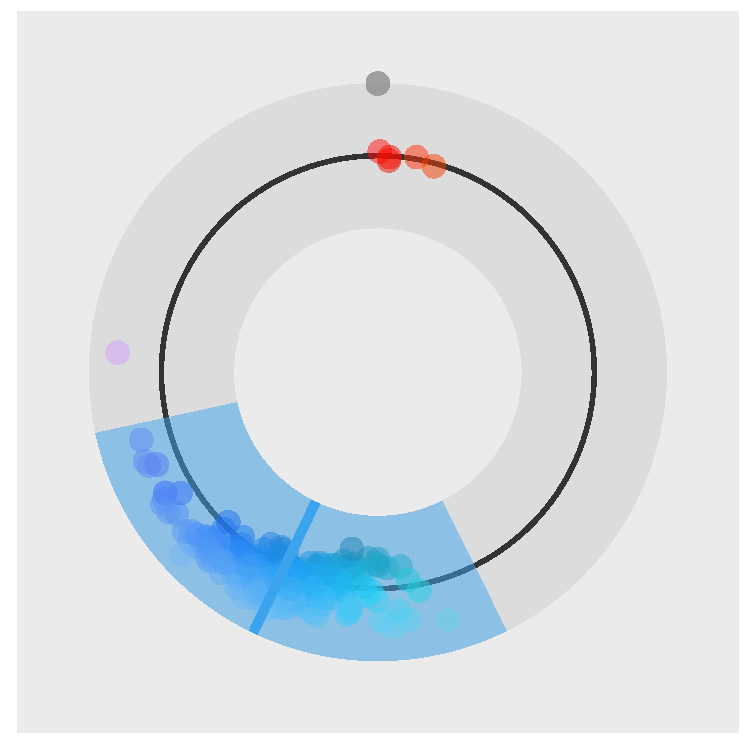
\includegraphics[width=\linewidth]{single_column.pdf}
	\caption{\textbf{A random visualization.} This is an example of a figure that spans only across one of the two columns.}
	\label{fig:column}
\end{figure}

On the other hand, \figurename~\ref{fig:whole} is an example of a figure that spans across the whole page (across both columns) of the report.

% \begin{figure*} makes the figure take up the entire width of the page
\begin{figure*}[ht]\centering
	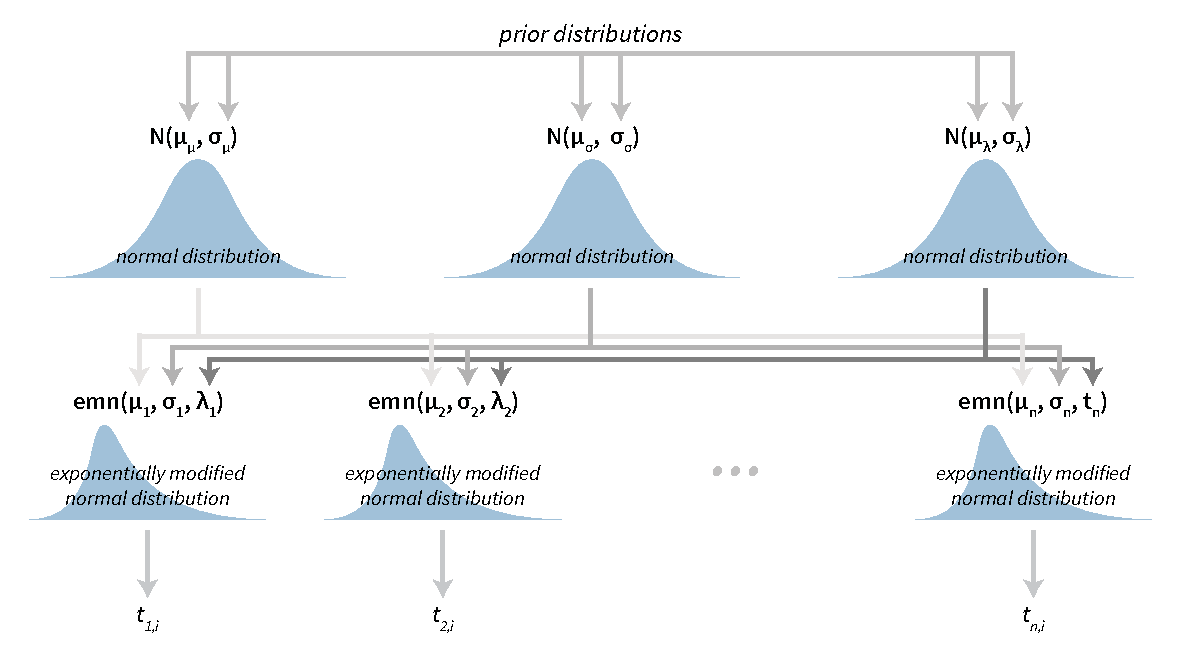
\includegraphics[width=\linewidth]{whole_page.pdf}
	\caption{\textbf{Visualization of a Bayesian hierarchical model.} This is an example of a figure that spans the whole width of the report.}
	\label{fig:whole}
\end{figure*}


\subsection*{Tables}

Use the table environment to insert tables.

\begin{table}[hbt]
	\caption{Table of grades.}
	\centering
	\begin{tabular}{l l | r}
		\toprule
		\multicolumn{2}{c}{Name}       \\
		\cmidrule(r){1-2}
		First name & Last Name & Grade \\
		\midrule
		John       & Doe       & $7.5$ \\
		Jane       & Doe       & $10$  \\
		Mike       & Smith     & $8$   \\
		\bottomrule
	\end{tabular}
	\label{tab:label}
\end{table}


\subsection*{Code examples}

You can also insert short code examples. You can specify them manually, or insert a whole file with code. Please avoid inserting long code snippets, advisors will have access to your repositories and can take a look at your code there. If necessary, you can use this technique to insert code (or pseudo code) of short algorithms that are crucial for the understanding of the manuscript.

\lstset{language=Python}
\lstset{caption={Insert code directly from a file.}}
\lstset{label={lst:code_file}}
\lstinputlisting[language=Python]{code/example.py}

\lstset{language=R}
\lstset{caption={Write the code you want to insert.}}
\lstset{label={lst:code_direct}}
\begin{lstlisting}
import(dplyr)
import(ggplot)

ggplot(diamonds,
	   aes(x=carat, y=price, color=cut)) +
  geom_point() +
  geom_smooth()
\end{lstlisting}

\end{comment}
%------------------------------------------------

\section*{Results}

\begin{comment}

Use the results section to present the final results of your work. Present the results in a objective and scientific fashion. Use visualisations to convey your results in a clear and efficient manner. When comparing results between various techniques use appropriate statistical methodology.

\subsection*{More random text}

This text is inserted only to make this template look more like a proper report. Lorem ipsum dolor sit amet, consectetur adipiscing elit. Etiam blandit dictum facilisis. Lorem ipsum dolor sit amet, consectetur adipiscing elit. Interdum et malesuada fames ac ante ipsum primis in faucibus. Etiam convallis tellus velit, quis ornare ipsum aliquam id. Maecenas tempus mauris sit amet libero elementum eleifend. Nulla nunc orci, consectetur non consequat ac, consequat non nisl. Aenean vitae dui nec ex fringilla malesuada. Proin elit libero, faucibus eget neque quis, condimentum laoreet urna. Etiam at nunc quis felis pulvinar dignissim. Phasellus turpis turpis, vestibulum eget imperdiet in, molestie eget neque. Curabitur quis ante sed nunc varius dictum non quis nisl. Donec nec lobortis velit. Ut cursus, libero efficitur dictum imperdiet, odio mi fermentum dui, id vulputate metus velit sit amet risus. Nulla vel volutpat elit. Mauris ex erat, pulvinar ac accumsan sit amet, ultrices sit amet turpis.

Phasellus in ligula nunc. Vivamus sem lorem, malesuada sed pretium quis, varius convallis lectus. Quisque in risus nec lectus lobortis gravida non a sem. Quisque et vestibulum sem, vel mollis dolor. Nullam ante ex, scelerisque ac efficitur vel, rhoncus quis lectus. Pellentesque scelerisque efficitur purus in faucibus. Maecenas vestibulum vulputate nisl sed vestibulum. Nullam varius turpis in hendrerit posuere.

Nulla rhoncus tortor eget ipsum commodo lacinia sit amet eu urna. Cras maximus leo mauris, ac congue eros sollicitudin ac. Integer vel erat varius, scelerisque orci eu, tristique purus. Proin id leo quis ante pharetra suscipit et non magna. Morbi in volutpat erat. Vivamus sit amet libero eu lacus pulvinar pharetra sed at felis. Vivamus non nibh a orci viverra rhoncus sit amet ullamcorper sem. Ut nec tempor dui. Aliquam convallis vitae nisi ac volutpat. Nam accumsan, erat eget faucibus commodo, ligula dui cursus nisi, at laoreet odio augue id eros. Curabitur quis tellus eget nunc ornare auctor.
\end{comment}

%------------------------------------------------

\section*{Discussion}


\begin{comment}
Use the Discussion section to objectively evaluate your work, do not just put praise on everything you did, be critical and exposes flaws and weaknesses of your solution. You can also explain what you would do differently if you would be able to start again and what upgrades could be done on the project in the future.
\end{comment}


%------------------------------------------------

\section*{Acknowledgments}

\begin{comment}
Here you can thank other persons (advisors, colleagues ...) that contributed to the successful completion of your project.
\end{comment}


%----------------------------------------------------------------------------------------
%	REFERENCE LIST
%----------------------------------------------------------------------------------------
\bibliographystyle{unsrt}
\bibliography{report}


\end{document}